\documentclass{article} % Класс печатного документа

% для поддержки русского языка
\usepackage[T2A]{fontenc} % поддержка специальных русских символов
\usepackage[utf8]{inputenc} % Кодировка исходного текста - utf8
\usepackage[english,russian]{babel} % Поддержка языка - русского с английским
\usepackage{indentfirst} % Отступ в первом абзаце

\usepackage{graphicx} % Для вставки картинок
\usepackage{hyperref} % Для вставки гиперссылок
\usepackage{listings} % Для вставки кусков кода
\usepackage{float} % Для точного позиционирования картинок
\usepackage{amsmath} % Для отключения нумерации у указанных формул
\usepackage{listings} % Добавление листингов
\usepackage[justification=centering]{caption} % для центрирования подписи к таблице

\title{Отчёт 5\\
Кластерный анализ с помощью метода k-средних} % заголовок документа
\author{Свичкарев А.\,В.} % Автор документа
\date{\today} % Текущая дата

\begin{document} % Конец преамбулы, начало текста

\maketitle % Печатает заголовок, список авторов и дату

\section*{Задачи}
Дана таблица 4 признаков для 150 экземпляров.

На основе набора данных требуется
выделить необходимое количество классов и
отнести каждый экземпляр к одному из них.

\clearpage
\section*{Выполнение}

Перед проведением кластеризации необходимо
выполнить стандартизацию данных,
так как шкалы признаков могут сильно отличаться.

Для определения оптимального числа кластеров
использовалась функция библиотеки NbClust.

\begin{figure}[H]
    \centering
    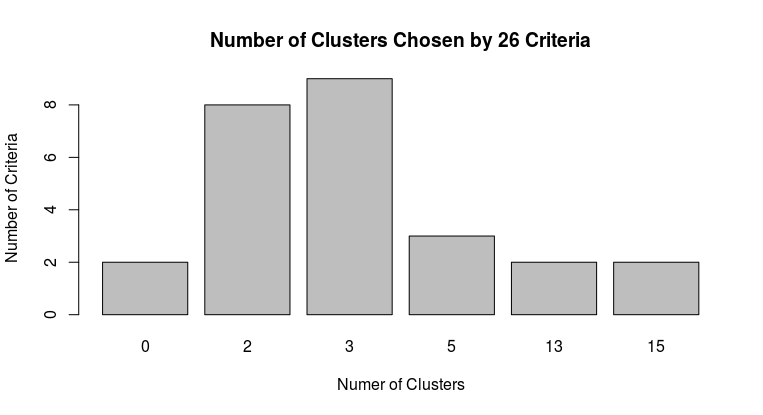
\includegraphics[width=\textwidth]{nclusters}
    \caption{Рекомендованное число кластеров
с использованием 26 критериев библиотеки NbClust}
\end{figure}

Для данной выборки можно выбрать 3 кластера,
хотя 2 кластера тоже приемлемо,
не такой большой отрыв.

Кластеризация проводилась с помощью
функции kmeans.
В качестве дополнительных аргументов
указывается выбранное число кластеров
и число запусков алгоритма.

Полученные центры кластеров
для стандартизированных данных
и для исходных:

\lstinputlisting[firstline=21,lastline=30]{task.log}

\clearpage
Таблица с приписанными номерами кластеров
у исходных экземпляров:

\lstinputlisting[firstline=36]{task.log}

\section*{Вывод}
Минусом данного метода кластеризации
является указания числа кластеров как параметра.

Алгоритм сильно зависит от начального
размещения кластеров,
поэтому нужно проводить много запусков
для получения хороших результатов.

Данный алгоритм хорошо подходит,
если у нас есть априорные знания
о числе кластеров и
их возможном расположение.

\section*{Исходный код}
Исходный код прилагается.

\end{document} % Конец документа
